\section{První týden}

\subsection{Důkaz souvislosti minima a maxima}

Tvrzení. Pro $f: D \rightarrow \R, M \subseteq D, \hat{x} \in M$ platí:

\begin{enumerate}[(1)]
    \item $\hat{x} \in \underset{x \in M}{\argmin} f(x) \iff \hat{x} \in \underset{x \in M}{\argmax} (-f(x))$,
    \item jesliže $\hat{x} \in \underset{x \in M}{\argmin} f(x)$, pak $\underset{x \in M}{\min} f(x) =
    - \underset{x \in M}{\max} (-f(x))$.
\end{enumerate}
Důkaz.

(1) $\hat{x} \in \underset{x \in M}{\argmin} f(x)$, tj. $f(\hat{x}) \leq f(x), \forall x \in M \underset{\cdot (-1)}{\iff}
-f(\hat{x}) \geq -f(x), \forall x \in M$, tj. $\hat{x} \in \underset{x \in M}{\argmax} (-f(x)). \qed$


(2) Ať $\hat{x} \in \underset{x \in M}{\argmin} f(x)$, pak $\underset{x \in M}{\min} f(x) = f(\hat{x}) =
- (- f(\hat{x})) \overset{(1)}{=} - \underset{x \in M}{\max} (-f(x)). \qed$

\subsection{Hledání přípustných množin}
\begin{align*}
    \text{minimalizujte } x^2 + 1 \\
    \text{za podmínek } \frac{3}{x} \leq 1, \\
    x \in \N.
\end{align*}
Upravíme podmínky a uděláme jejich průnik: $(x - 3 \geq 0) \land (x \in \N) \Rightarrow M = \N \setminus \bc{1,2}$.

Úvahou pak lze uhodnout minimum - minimum leží v bodě $x=3$.

\subsection{Hledání přípustných množin}
\begin{align*}
    \text{maximalizujte } \ln x \\
    \text{za podmínek } x \leq 5, \\
    \cos(\pi x) = 1.
\end{align*}
$D(f) = (0, \infty)$.

Udělejme průnik definičního oboru funkce a podmínek: $(x \in (0, \infty)) \land (x \leq 5) \land (\cos(\pi x)=1)$.

\begin{multicols}{2}
    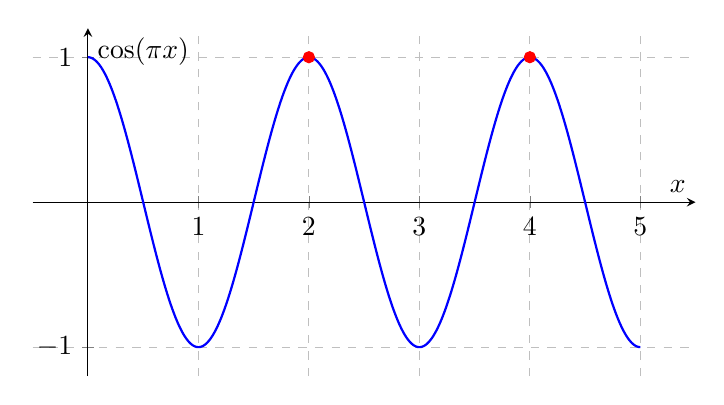
\begin{tikzpicture}
        \begin{axis}[
            axis lines = middle,
            xlabel = $x$,
            ylabel = {$\cos(\pi x)$},
            domain=0:5,
            samples=1000,
            %   xtick={0,1,2,3,4,5},
            %   ytick={-1,-0.5,0,0.5,1},
            enlargelimits,
            grid=both,
            minor grid style={dotted},
            major grid style={dashed},
            width=10cm, height=6cm,
        ]
            \addplot[blue, thick] {cos(deg(x * pi))};
            \addplot[only marks, red, mark=*] coordinates {(2,1) (4,1)};
        \end{axis}
      \end{tikzpicture}
\columnbreak

      \quad Očividně tedy $M = \bc{2,4}$.

      \quad Úvahou pak lze uhodnout $\underset{x \in M}{\argmax} \ln x = \bc{4}$.
\end{multicols}

\subsection{Maximalisační úloha}
Banka nabízí dva investiční produkty. Očekávaný měsíční výnos prvního investičního produktu (v tis. Kč) při investici $x$
(v tis. Kč) je $\frac{2x}{4x+25}$ a očekávaný měsíční výnos druhého invetičního produktu (v tis. Kč) při investici $x$
(v tis. Kč) je $\frac{x}{x+50}$. Jakým způsobem má investor rozdělit částku $c = 100000$ Kč mezi uvedené dva produkty tak,
aby celkový očekávaný měsíční výnos byl co největší?

\subsection{Minimalisační úloha}
Ve firmě potřebují nalézt rozměry otevřené krabice (tj. krabice bez horní stěny) se čtvercovou podstavou o objemu $10$
d$\text{m}^3$ tak, aby obsah plochy jejího pláště byl co nejmenší. Formulujte odpovídající optimalisační úlohu za
předpokladu, že krabice je vyrobena z materiálu, jehož tloušťka je zanedbatelná. Tuto úlohu poté vyřešte.

\subsection{Maximalisační úloha}
V továrně vyrábějí zboží různých druhů. Označme je $X_1, \dots, X_n$. Na jejich výrobu potřebují materiály $Y_1, \dots, Y_m$.
Na skladě mají k dispozici množství $b_i$ materiálu $Y_i$ a na trhu ho nakupují za cenu $\gamma_i$. Na výrobu jednotkového
množství zboží $X_j$ potřebují množství $a_{ij}$ materiálu $Y_i$. Jednotkové množství výrobku $X_j$ prodávají za cenu
$\sigma_j$. Formulujte optimalisační úlohu problému nastavení množství výroby jednotlivých druhů produktů (předpokládejte,
že hledaná množství nemusí být celočíselná) tak, aby celkový zisk z jejich prodeje byl co největší.

\subsection{Optimalisační úloha s nadrovinami}
V $\R^n$ jsou dány množiny bodů $A = \bc{a_1, \dots, a_k}$ a $B = \bc{b_1, \dots, b_t}$. Ať $w \in \R^n$ a $\lambda \in \R$.
Předpokládejme, že $H$ je nadrovina o rovnici $\langle x,w \rangle + \lambda = 0$, $H_1$ je nadrovina o rovnici
$\langle x, w \rangle + \lambda = 1$ a $H_2$ je nadrovina o rovnici $\langle x, w \rangle + \lambda = -1$.
\begin{enumerate}[(a)]
    \item Ukažte, že vzdálenost mezi nadrovinami $H_1$ a $H_2$ je $\frac{2}{||w||}$. Dále ukažte, že $\frac{1}{||w||}$
    je vzdálenost $H$ od $H_1$ a také vzdálenost $H$ od $H_2$.
    \item Iterpretujte optimalisační úlohu
    \begin{align*}
        \text{maximalisujte } & g(w, \lambda) = \frac{2}{||w||} \\
        \text{za podmínek }   & \langle a_i, w \rangle + \lambda \geq 1 \text{ pro všechna } i=1, \dots, k, \\
                              & \langle b_i, w \rangle + \lambda \leq -1 \text{ pro všechna } j=1, \dots, l.
    \end{align*}
    \item Ukažte, že $(\hat w,\hat \lambda)$ je řešením úlohy z předchozího bodu právě tehdy, když je řešením úlohy
    (kvadratického programování) ve tvaru
    \begin{align*}
        \text{minimalisujte } & h(w, \lambda) = \frac{1}{2} ||w||^2 \\
        \text{za podmínek }   & \langle a_i, w \rangle + \lambda \geq 1 \text{ pro všechna } i=1, \dots, k, \\
                              & \langle b_i, w \rangle + \lambda \leq -1 \text{ pro všechna } j=1, \dots, l.
    \end{align*}
\end{enumerate}

\subsection{Optimalisační úloha se spojnicemi bodů}
V rovině jsou dány body $P = (0,0)^T$ a $Q = (1,1)^T$.
\begin{enumerate}[(a)]
    \item Formulujte optimalisační úlohu problému nalezení nejkratší spojnice bodů $P$ a $Q$. Spojnicí rozumíme křivku
    danou grafem spojitě diferencovatelné funkce $f : [0,1] \rightarrow \R$.
    \item Nalezněte řešení úlohy z předchozího bodu.\footnote{Nápověda: Ukažte, že $g(t) = t, t \in [0,1]$, je řešením
    úlohy. Využijte přitom toho, že pro dvě spojité funkce $f_1$ a $f_2$ na intervalu $[0,1]$ je $\int_0^1 \left(f_1(t),
    f_2(t) \right)^T \dif T := \left(\int_0^1 f_1 (t) \dif t, \int_a^b f_2 (t) \dif t \right)^T$ a platí \\
    $\left| \left| \int_0^1 (f_1 (t), f_2 (t))^T \dif t \right| \right| \leq \int_0^1 \left| \left| (f_1 (t), f_2 (t))^T \right| \right| \dif t$.
    K důkazu jednoznačnosti pak lze využít tvrzení, že rovnost v uvedené \uv{trojúhelníkové nerovnosti pro integrály}
    nastává pávě tehdy, když existuje spojitá funkce $\lambda : [0,1] \rightarrow \R$ taková, že $(f_1 (t), f_2 (t))^T =
    \lambda (t) \int_0^1 (f_1 (t), f_2 (t))^T \dif t$.
    }
\end{enumerate}

\subsection{Optimalisační úloha s úsečkami}
V rovině jsou dány body $P = (-1, 0)^T$ a $Q = (1,0)^T$. Ať $L$ je úsečka s krajními body $P$ a $Q$.
\begin{enumerate} [(a)]
    \item Formulujte optimalisační plohu problému nalezení spojitě diferencovatelné funkce $y : [-1, 1] \rightarrow \R$,
    jejíž graf má koncové body $P$ a $Q$, délku $l=3$, leží v horní polorovině a spolu s úsečkou $L$ ohraničuje část
    roviny o největším obsahu.
    \item Ať $(x_0, x_1, \dots, x_k)$ je ekvidistantní dělení intervalu $[-1, 1]$ (tj. $x_l = l \delta$, kde
    $\delta = \frac{2}{k}$). Využitím tohoto dělení k aproximaci integrálu pomocí konečné sumy a derivace pomocí diferencí
    nalezněte optimalisační úlohu v $\R^{k+1}$, jejíž řešení aproximuje řešení úlohy z předchozího bodu.
\end{enumerate}

\subsection{Vztah argmin}
Ať $\varphi : X \rightarrow Y$ je bijekce, $D_f \subseteq X, D_g \subseteq Y, \varphi(D_f) \subseteq D_g, M \subseteq D_f$
a $\hat x \in M$. Předpokládejme, že funkce $f : D_f \rightarrow \R$ a $g : D_g \rightarrow \R$ splňují $f = g \circ \varphi$.
Ukažte, že $\hat x \in \argmin_{x \in M} f(x)$ právě tehdy, když $\varphi (\hat x) \in \argmin_{y \in \varphi (M)} g(y)$.

\newpage
\section*{Konvexní množiny} \label{sec:konvex}
Definice. Množina $C \subseteq \R^n$ se nazve konvexní, jestliže pro každé $x, y \in C$ je $[x,y] \in C$.

\subsection{Uzavřená úsečka}
Nechť $x, y \in \R^n$. Množina
\[ [x,y] := \bc{\lambda x + (1-\lambda)y \mid 0 \leq \lambda \leq 1} \]
se nazývá uzavřená úsečka s krajními body $x$ a $y$.

\subsection{Je nadrovina konvexní?}
Definice nadroviny: $H(y; \alpha) := \bc{x \in \R^n \mid \langle x, y \rangle = \alpha}$, $y \in \R^n$, $\alpha \in \R$.

Důkaz.

Ať $x,z \in H(y, \alpha), \lambda \in [0,1]$.\\
Cíl: $\lambda x + (1-\lambda) z \in H(y, \alpha)$. Tedy dokazujeme podle \hyperref[sec:konvex]{definice}.

$\langle \lambda x + (1-\lambda)z, y \rangle = \lambda \underbrace{\langle x,y \rangle}_{\alpha} + (1-\lambda)
\underbrace{\langle z,y \rangle}_{\alpha} = \lambda \alpha + (1-\lambda) \alpha = \alpha$.

$\Rightarrow \lambda x + (1-\lambda)z \in H(y, \alpha). \qed$

\subsection{Je uzavřený poloprostor konvexní?}

\subsection{Je uzavřená koule konvexní?}
Definice uzavřené koule: $B(a,r) = \bc{a \in \R^n \mid ||x -a || \leq r}$, o středu $a \in \R^n$ a poloměru $r > 0$.

Důkaz.

Ať $x,y \in \R^n, \lambda \in [0,1]$.\\
Cíl: $|| [\lambda x + (1-\alpha)y] - a || \leq r$. Tedy za $x$ z definice dosadíme úsečku mezi body $x$ a $y$, které jsme
si vybrali a chceme ukázat, že i tato úsečka leží v uzavřené kouli, dle \hyperref[sec:konvex]{definice}.

\[
    || [\lambda x + (1-\alpha)y] - a || = || \lambda x - (1-\lambda)a + (1-\lambda)y - \lambda a || =
    || \lambda (x-a) + (1-\lambda)(y-a) ||
\]
\[
    \leq \lambda ||\underbrace{x-a}_{\leq r}|| +  (1-\lambda)||\underbrace{y-a}_{\leq r}|| \leq \lambda r + (1-\lambda)r
     = r. \qed
\]

\subsection{Je okolí konvexní?}
Definice okolí: $B(a,r) = \bc{a \in \R^n \mid ||x -a || < r}$, o středu $a \in \R^n$ a poloměru $r > 0$.

Důkaz.

Ať $x,y \in \R^n, \lambda \in [0,1]$.\\
Cíl: $|| [\lambda x + (1-\alpha)y] - a || < r$. Dle \hyperref[sec:konvex]{definice}.

\[
    || [\lambda x + (1-\alpha)y] - a || = || \lambda x - (1-\lambda)a + (1-\lambda)y - \lambda a || =
    || \lambda (x-a) + (1-\lambda)(y-a) ||
\]
\[
    \leq \lambda ||\underbrace{x-a}_{< r}|| +  (1-\lambda)||\underbrace{y-a}_{< r}|| < \lambda r + (1-\lambda)r
     = r. \qed
\]

\subsection{Je průnik množin konvexní?}
Úvaha pro 2 množiny ve $\R^2$:

\begin{multicols}{2}
    Mějme jednu modrou ($y \geq 0$) a druhou červenou ($x \geq 0$) \hyperref[sec:konvex]{konvexní} množinu. Jejich průnik je pak nezáporný ortant,
    tedy \\
    $\R_+^n = \bc{(x_1, \dots, x_n)^T \in \R^n \mid x_1 \geq 0, \dots, x_n \geq 0}$.

    Visuálně je průnik nekonvexní.

    Důkaz.

    Nechť ${x,y \in \bigcap\limits_{i \in I} \M_{i}, \forall i \in I \implies [x, y] \in \M_i, \forall i \in I
    \implies [x,y] \subseteq \bigcap\limits_{i \in I} \M_{i}.}$
    $\qed$

\columnbreak

    \begin{center}
        \begin{tikzpicture}
            % y > 0 ("/")
            \fill[pattern=north east lines, pattern color=blue, opacity=0.6] (-2,0) rectangle (2,2);

            % x > 0 ("\")
            \fill[pattern=north west lines, pattern color=red, opacity=0.6] (0,-2) rectangle (2,2);

            \draw[thick,->] (-2.2,0) -- (2.2,0) node[anchor=north] {\(x\)};
            \draw[thick,->] (0,-2.2) -- (0,2.2) node[anchor=east] {\(y\)};

            % \foreach \x in {-4,-3,-2,-1,1,2,3,4}
            %     \draw[dashed, gray] (\x,-4) -- (\x,4);
            % \foreach \y in {-4,-3,-2,-1,1,2,3,4}
            %     \draw[dashed, gray] (-4,\y) -- (4,\y);

            \node[anchor=north east] at (0,0) {\(0\)};
        \end{tikzpicture}
    \end{center}
\end{multicols}

\subsection{Důkaz, že rozdíl a sjednocení nezachovává konvexitu}
Mějme $[0,1] \setminus (0,1) = \bc{0,1} = \bc{0} \cup \bc{1}$.

$[0,1]$ a $(0,1)$ jsou \hyperref[sec:konvex]{konvexní} množiny. Jejich rozdíl ale už konvexní není.\\
$\bc{0}$ a $\bc{1}$ jsou konvexní množiny. Jejich sjednocení ale už konvexní není.

\section*{Afinní zobrazení} \label{sec:afin}
Definice. Zobrazení $f: \R^n \rightarrow \R^m$ se nazývá afinní, existují-li $A \in \M_{m,n} (\R)$ a $b \in R^m$
tak, že $f(x) = Ax + b$.

\subsection{Důkaz, že afinní zobrazení je konvexní}
Tvrzení.

Nechť $f: \R^n \rightarrow \R^m$. Pak $f$ je \hyperref[sec:afin]{afinní} $\iff$ pro každé $x,y \in \R^n$ a každé
$\lambda \in \R$ platí
\[f(\lambda x + (1-\lambda) y) =\lambda f(x) + (1-\lambda) f(y)\text{.}\]

Důkaz.

"$\Rightarrow$": Ať $f(x) = Ax + b$, kde $A \in \M_{m,n} (\R)$, $b \in \R^n$.

Ať $x, y \in \R^n, \lambda \in \R$.
\[
    f(\lambda x + (1 - \lambda) y) = A [\lambda x + (1-\lambda) y] + b = \lambda A x + (1-\lambda)Ay + \lambda b +
    (1-\lambda)b =
\]
\[
    \lambda \underbrace{(Ax + b)}_{f(x)} + (1-\lambda)\underbrace{(Ay + b)}_{f(y)} = \lambda f(x) + (1-\lambda)f(y). \qed
\]

"$\Leftarrow$":
Cíl: Ukázat, že $f$ je \hyperref[sec:afin]{afinní}, tedy $f(x) = Ax + b$.\\
Zvolme $\varphi(x) = f(x) - f(0)$.\\
Pokud je $f$ \hyperref[sec:afin]{afinní}, pak zobrazení $\varphi$ by mělo být dáno jako $Ax$, tedy být lineární.\\
Cíl: $\varphi$ je lineární zobrazení.

Musíme ověřit uzavřenost na násobení a sčítání z definice.

(1) Ať $x \in \R^n$, $\alpha \in R$.\\
Cíl: $\varphi(\alpha x) = \alpha \varphi(x)$.
\[
    \varphi(\alpha x) = f(\alpha x) - f(0) = f(\alpha x + (1-\alpha)0) - f(0) = \alpha f(x) + (1-\alpha)f(0) - f(0) =
\]
\[
    \alpha f(x) - \alpha f(0) = \alpha (f(x) - f(0)) = \alpha \varphi (x-0). \qed
\]

(2) Ať $x, y \in \R^n$.\\
Cíl: $\varphi(x+y) = \varphi(x) + \varphi(y)$.
\[
    \varphi(x+y) = \varphi \left(2 \left(\frac{1}{2} (x+y)\right)\right) \stackrel{(1)}{=} 2 \varphi \left(\frac{1}{2} (x+y)\right) =
    2 \left[f(\frac{1}{2}x + \frac{1}{2}y) - f(0)\right] = 2 \left[\frac{1}{2} f(x) + \frac{1}{2}f(y) - f(0) \right] =
\]
\[
    f(x) + f(y) - f(0) - f(0) = \underbrace{f(x) - f(0)}_{\varphi(x)} + \underbrace{f(y) - f(0)}_{\varphi(y)} =
    \varphi(x) + \varphi(y). \qed
\]

\subsection{Důkaz, že obraz konvexní množiny při afinním zobrazení je konvexní}
Tvrzení.

Je-li $f: \R^n \rightarrow \R^m$ \hyperref[sec:afin]{afinní} a $C \subseteq \R^n$ \hyperref[sec:konvex]{konvexní}, pak
$f(C)$ je konvexní.

Důkaz.

Mějme $a, b \in f(C) \implies \exists x, y \in C: f(x)=a, f(y)=b$.

Dle předpokladu je $C$ konvexní. $\implies [x, y] \subseteq C \implies \underbrace{f([x, y])}_{\subseteq f(C)} =
[\underbrace{f(x)}_a, \underbrace{f(y)}_b] \subseteq f(C). \qed$

\subsection{Důkaz, že kartézský součin je konvexní}
Tvrzení.

Nechť $C_1 \subseteq \R^n$ a $C_2 \subseteq \R^m$. Pak $C_1$ a $C_2$ jsou \hyperref[sec:konvex]{konvexní} množiny právě tehdy, když
$C_1 \bigtimes C_2$ je konvexní množina.

Důkaz.

"$\Rightarrow$": Mějme
$
\begin{bmatrix}
    a \\
    b
\end{bmatrix}\hspace{-1mm}\text{,}
\begin{bmatrix}
    c \\
    d
\end{bmatrix} \in C_1 \bigtimes C_2, \lambda \in [0,1]$\\
Cíl:
$
\lambda \begin{bmatrix}
    a \\
    b
\end{bmatrix}
+ (1-\lambda)
\begin{bmatrix}
    c \\
    d
\end{bmatrix} \in C_1 \bigtimes C_2.$ Dle \hyperref[sec:konvex]{definice}.

$
\lambda \begin{bmatrix}
    a \\
    b
\end{bmatrix}
+ (1-\lambda)
\begin{bmatrix}
    c \\
    d
\end{bmatrix} =
\begin{bmatrix}
    \lambda a \\
    \lambda b
\end{bmatrix}
+
\begin{bmatrix}
    (1-\lambda)c \\
    (1-\lambda)d
\end{bmatrix}
=
\begin{bmatrix} % TODO: add overbrace?
    \lambda a + (1-\lambda)c \\
    \lambda b + (1-\lambda)d
\end{bmatrix} \in C_1 \bigtimes C_2. \qed$

"$\Leftarrow$": Definujme \hyperref[sec:afin]{afinní} zobrazení $f : \R^n \times \R^m \rightarrow \R^n$ předpisem
\[ f(x,y) = x \text{.}\]
Pak $f$ je afinní. Navíc $f(C_1 \bigtimes C_2) = C_1$. $\implies C_1$ je \hyperref[sec:konvex]{konvexní}, protože afinní
zobrazení zachovává konvexitu.
A důkaz bude obdobný pro $C_2$, zde zadefinujme afinní zobr. $g : \R^n \times \R^m \rightarrow \R^n$ předpisem
\[ g(x,y) = y \text{.}\]
Pak $g$ je afinní. Navíc $g(C_1 \bigtimes C_2) = C_2$. $\implies C_2$ je konvexní, protože afinní zobrazení zachovává
konvexitu. $\qed$

\subsection{Práce s ortonormální bází a skalárním součinem}
Uvažme lineární prostor $\S^n = \bc{A \in \M_n (\R) \mid A^ T = T}$ reálných symetrických $n \times n$
matic se skalárním součinem $\langle A B \rangle _{\S_n} = Tr (AB)$.
\begin{enumerate}[(a)]
    \item Ukažte, že $
    \begin{bmatrix}
        \begin{pmatrix}
            1 & 0 \\
            0 & 0
        \end{pmatrix},
        & \frac{1}{\sqrt{2}}
        \begin{pmatrix}
            0 & 1 \\
            1 & 0
        \end{pmatrix},
        &
        \begin{pmatrix}
            0 & 0 \\
            0 & 1
        \end{pmatrix}
    \end{bmatrix}$
    je ortonormální báze na $\S^2$.
    \item Ukažte, že zobrazení
    \[ \varphi:
    \begin{bmatrix}
        a & b \\
        b & c
    \end{bmatrix} \in \S^2 \mapsto
    \begin{bmatrix}
        a \\
        \sqrt{2}b \\
        c
    \end{bmatrix} \in \R^3
    \]
    je isomorfismus lineárního prostoru $\S^2$ na $\R^3$ zachovávající skalární součin (tj. \\ $\langle A, B \rangle _{\S_2} = \langle \varphi(A), \varphi(B) \rangle$ pro všechna $A,B \in
    \S^2$, kde $\langle \dots \rangle$ je standardní skalární součin na $\R^3$)
    \item Zobecněte výsledky bodů (a) a (b) do prostoru $\S^2 na \R^2$ zachovávající skalární součin.
    \item Ať $\S^2_+$ je množina všech reálných symetrických $2 \times 2$ matic, které jsou navíc positivně
    semidefinitní. Ukažte, že jestliže $\varphi$ je zobrazení z bodu (b), pak
    \[\varphi(\S^2_+) = \bc{(x,y,z)^T \in \R^3 \mid x \geq 0, z \geq 0, 2xz - y^2 \geq 0} \text{.}\]
\end{enumerate}

\subsection{Bijekce mezi dvěma optimalisačními úlohami}
Je dána úloha
\begin{align*}
    \text{minimalisujte } & \langle X, A \rangle _{\S_2} \\
    \text{za podmínek }   & \langle X, \bb{1} \rangle _{\S_2} = 2, \\
                          & X \in \S_+^2,
\end{align*}
kde $A =
    \begin{bmatrix}
        3 & 1 \\
        1 & 1
    \end{bmatrix}
$ a $\bb{1} =
    \begin{bmatrix}
        1 & 0 \\
        0 & 1
    \end{bmatrix}
$. Ukažte\footnote{Nápověda: využijte výsledků 7. a 8. příkladu.}, že existuje bijekce mezi množinou všech jejich řešení a množinou všech řešení úlohy
\begin{align*}
    \text{minimalisujte } & 3x_1 + 2x_2 + x_3 \\
    \text{za podmínek }   & x_1 + x_3 = 2, \\
                          & x_1 x_3 - x_2^2 \geq 0,
                          & x_1, x_3 \geq 0.
\end{align*}

\subsection{Bijekce mezi dvěma optimalisačními úlohami}
Je dána úloha
\begin{align*}
    \text{minimalisujte } & \langle X, A \rangle _{\S_2} \\
    \text{za podmínek }   & \langle X, B \rangle _{\S_2} = 0, \\
                          & \langle X, \bb{1} \rangle _{\S_2} = 1, \\
                          & X \in \S_+^2,
\end{align*}
kde $A =
    \begin{bmatrix}
        2 & 0 \\
        0 & -1
    \end{bmatrix}
$, $B =
    \begin{bmatrix}
        0 & 1 \\
        1 & 0
    \end{bmatrix}
$ a $\bb{1} =
    \begin{bmatrix}
        1 & 0 \\
        0 & 1
    \end{bmatrix}
$. Ukažte\footnote{Nápověda: využijte výsledků 7. a 8. příkladu.}, že existuje bijekce mezi množinou všech jejich řešení a množinou všech řešení úlohy
\begin{align*}
    \text{minimalisujte } & 2x-y \\
    \text{za podmínek }   & x+y=1, \\
                          & x, y \geq 0.
\end{align*}

\subsection{Určení definitnosti matic}
Určete definitnost matice $A$, jestliže
\begin{enumerate}[(a)]
    \item
    $\begin{bmatrix}
        9 & 6 \\
        6 & 4
    \end{bmatrix}$;
    \item
    $\begin{bmatrix}
        15 & 3 & 2 \\
        3 & 1 & 0 \\
        2 & 0 & 1
    \end{bmatrix}$;
    \item
    $\begin{bmatrix}
        4 & 2 & 2 \\
        2 & 1 & 1 \\
        2 & 1 & 0
    \end{bmatrix}$;
    \item
    $\begin{bmatrix}
        3 & 2 & 1 \\
        2 & 1 & 1 \\
        1 & 1 & 0
    \end{bmatrix}$;
    \item
    $\begin{bmatrix}
        -1 & 0 & 1 \\
        0 & -2 & 2 \\
        1 & 2 & -3
    \end{bmatrix}$;
    \item
    $\begin{bmatrix}
        1 & 2 & 0 \\
        2 & 5 & 1 \\
        0 & 1 & 1
    \end{bmatrix}$.
\end{enumerate}

\subsection{Existence matice}
Ať $A \in \M_n (\R)$.
\begin{enumerate}[(a)]
    \item Ukažte, že $\langle Ax, y \rangle = \langle x, A^T y \rangle$ pro všechna $x, y \in \R^n$.
    \item Ukažte, že existují matice $B, C \in \M_n (\R)$ takové, že $B^T = B$, $C^T = -C$ a $A = B + C$. Jsou
    matice $B$ a $C$ určeny jednoznačně?
    \item Ukažte, že existuje symetrická matice $B \in \M_n (\R)$ taková, že $\langle Ax, x \rangle =
    \langle Bx, x \rangle$.
\end{enumerate}

\subsection{Gradient vektorového součinu}
Nalezněte $\nabla f(x)$ a $\nabla^2 f(x)$, jestliže
\begin{enumerate}[(a)]
    \item $f(x) = \langle x,c \rangle$, kde $c \in \R^n$;
    \item $f(x) = \langle Ax, x \rangle$, kde $A \in \M_n (\R)$. Určete také $\nabla f(x)$ a $\nabla^2 f (x)$ za
    dodatečného předpokladu, že $A$ je symetrická matice.
\end{enumerate}